\documentclass[runningheads,a4paper]{llncs}

\usepackage{url}
\usepackage{graphicx}
\newcommand{\keywords}[1]{\par\addvspace\baselineskip
\noindent\keywordname\enspace\ignorespaces#1}

\begin{document}
    \graphicspath{ {../img/} }
    \mainmatter

    \title{Proposal for Bachelor Thesis}
    \subtitle{A Sliding Window Filter for Time Series Streams\\
    \textnormal{\small{Supervisor: Stephan Spiegel\\\vspace{1\baselineskip}}}}

    \titlerunning{Proposal for bachelor thesis}

    \author{Gordon Lesti\\313249\\Course of studies: Bachelor of Computer Science\\gordon.lesti@campus.tu-berlin.de\\\vspace{5\baselineskip}}

    \authorrunning{Gordon Lesti}

    \institute{Technische Universit\"at Berlin\\
    Fakult\"at IV Elektrotechnik und Informatik\\
    Fachgebiet AOT\\
    Prof. Dr. Sahin Albayrak\\
    \url{http://www.aot.tu-berlin.de/}}

    \toctitle{Proposal for bachelor thesis}
    \tocauthor{Gordon Lesti}
    \maketitle
    \newpage

    \section{Introduction}
    % 3-5 Absätze
    % Allgemeine Einleitung
    % Lücke wurde schon identifiziert?
    % Bisherige Ansätzte
    % Eigener Vorschlag
    % Struktur der Bachelorarbeit / Zeitplan

    \section{Problem Description}
    % informelle & formelle Problembeschreibung

    \section{Objectives}
    % Eigener Ansatz

    \section{Evaluation}
    % Beschreibung des Datensatzes (uWave)

    \subsection{Experiment}
    I have created a experiment to record the acceleration data from a Wii Remote controller that is used by a
    experimentee to perform gestures mixed with physical activity. A experimentee has to perform a number of tasks. The
    tasks are a mix of physical activity and performing gestures. Figure~\ref{fig:wii-remote} shows a Wii Remote Plus
    controller.

    \begin{figure}
        \centering
        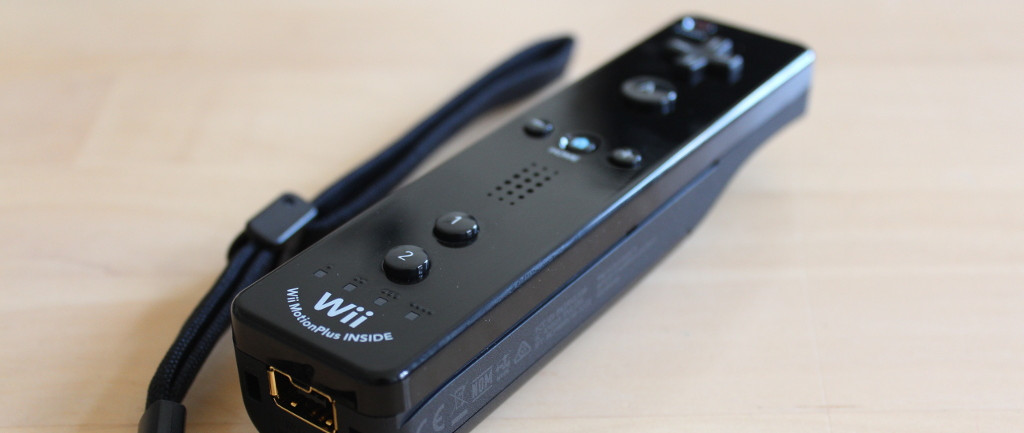
\includegraphics[width=0.9\textwidth]{wii-remote-plus.jpg}
        \caption{A black Wii Remote Plus controller.}
        \label{fig:wii-remote}
    \end{figure}

    \subsubsection{Implementation of the experiment}
    The program that is running the experiment is implemented in the programming language Python and available on
    GitHub\footnote{https://github.com/GordonLesti/SlidingWindowFilter-experiment}. The requirements to run the
    experiment are Python 2\footnote{https://www.python.org/}, xwiimote\footnote{https://github.com/dvdhrm/xwiimote} and
    xwiimote-bindings\footnote{https://github.com/dvdhrm/xwiimote-bindings}.

    \subsubsection{Course of the experiment}
    As mentioned above, one instance of the experiment will be performed with one experimentee and a Wii Remote
    controller. The tasks of the experiment will be communicated to the experimentee by a row of different screens that
    are changing after every gesture. Here are the rules of the experiment that will be explained to the experimentee
    before it begins.
    \begin{itemize}
        \item The Wii controller must be held in the same hand all the time during the hole experiment.
        \item The \textit{B} button of the controller is the trigger on the bottom of the controller.
        \item A gesture has to be performed by pressing the \textit{B} button down, holding the button, performing the
        gesture simultaneously and releasing the button after the gesture.
        \item It is not allowed to push the \textit{B} button outside of a gesture that is demanded by the experiment.
    \end{itemize}

    \paragraph{Task screens} are just images that are changing like a presentation after every gesture performed by the
    experimentee. The screens are shown in figure~\ref{fig:screens} and have the following functions.
    \begin{itemize}
        \item Screen \textit{(a)} is just welcoming the experimentee.
        \item Screen \textit{(b)} to \textit{(i)} are only for training gestures recordings.
        \item Screen \textit{(j)} to \textit{(q)} containing a physical activity followed by a gesture.
        \item Screen \textit{(r)} is just thanking the experimentee.
        \item Screen \textit{(s)} is just closing the experiment.
    \end{itemize}
    The program that is running during the experiment is recording the acceleration data from the Wii Remote controller
    all the time. Also the button down event of the \textit{B} button and the button up event will be recorded. The
    program will switch to the next task screen after every button up event, means after every gesture.

    \begin{figure}
        \centering
        \begin{tabular}{ccc}
            \frame{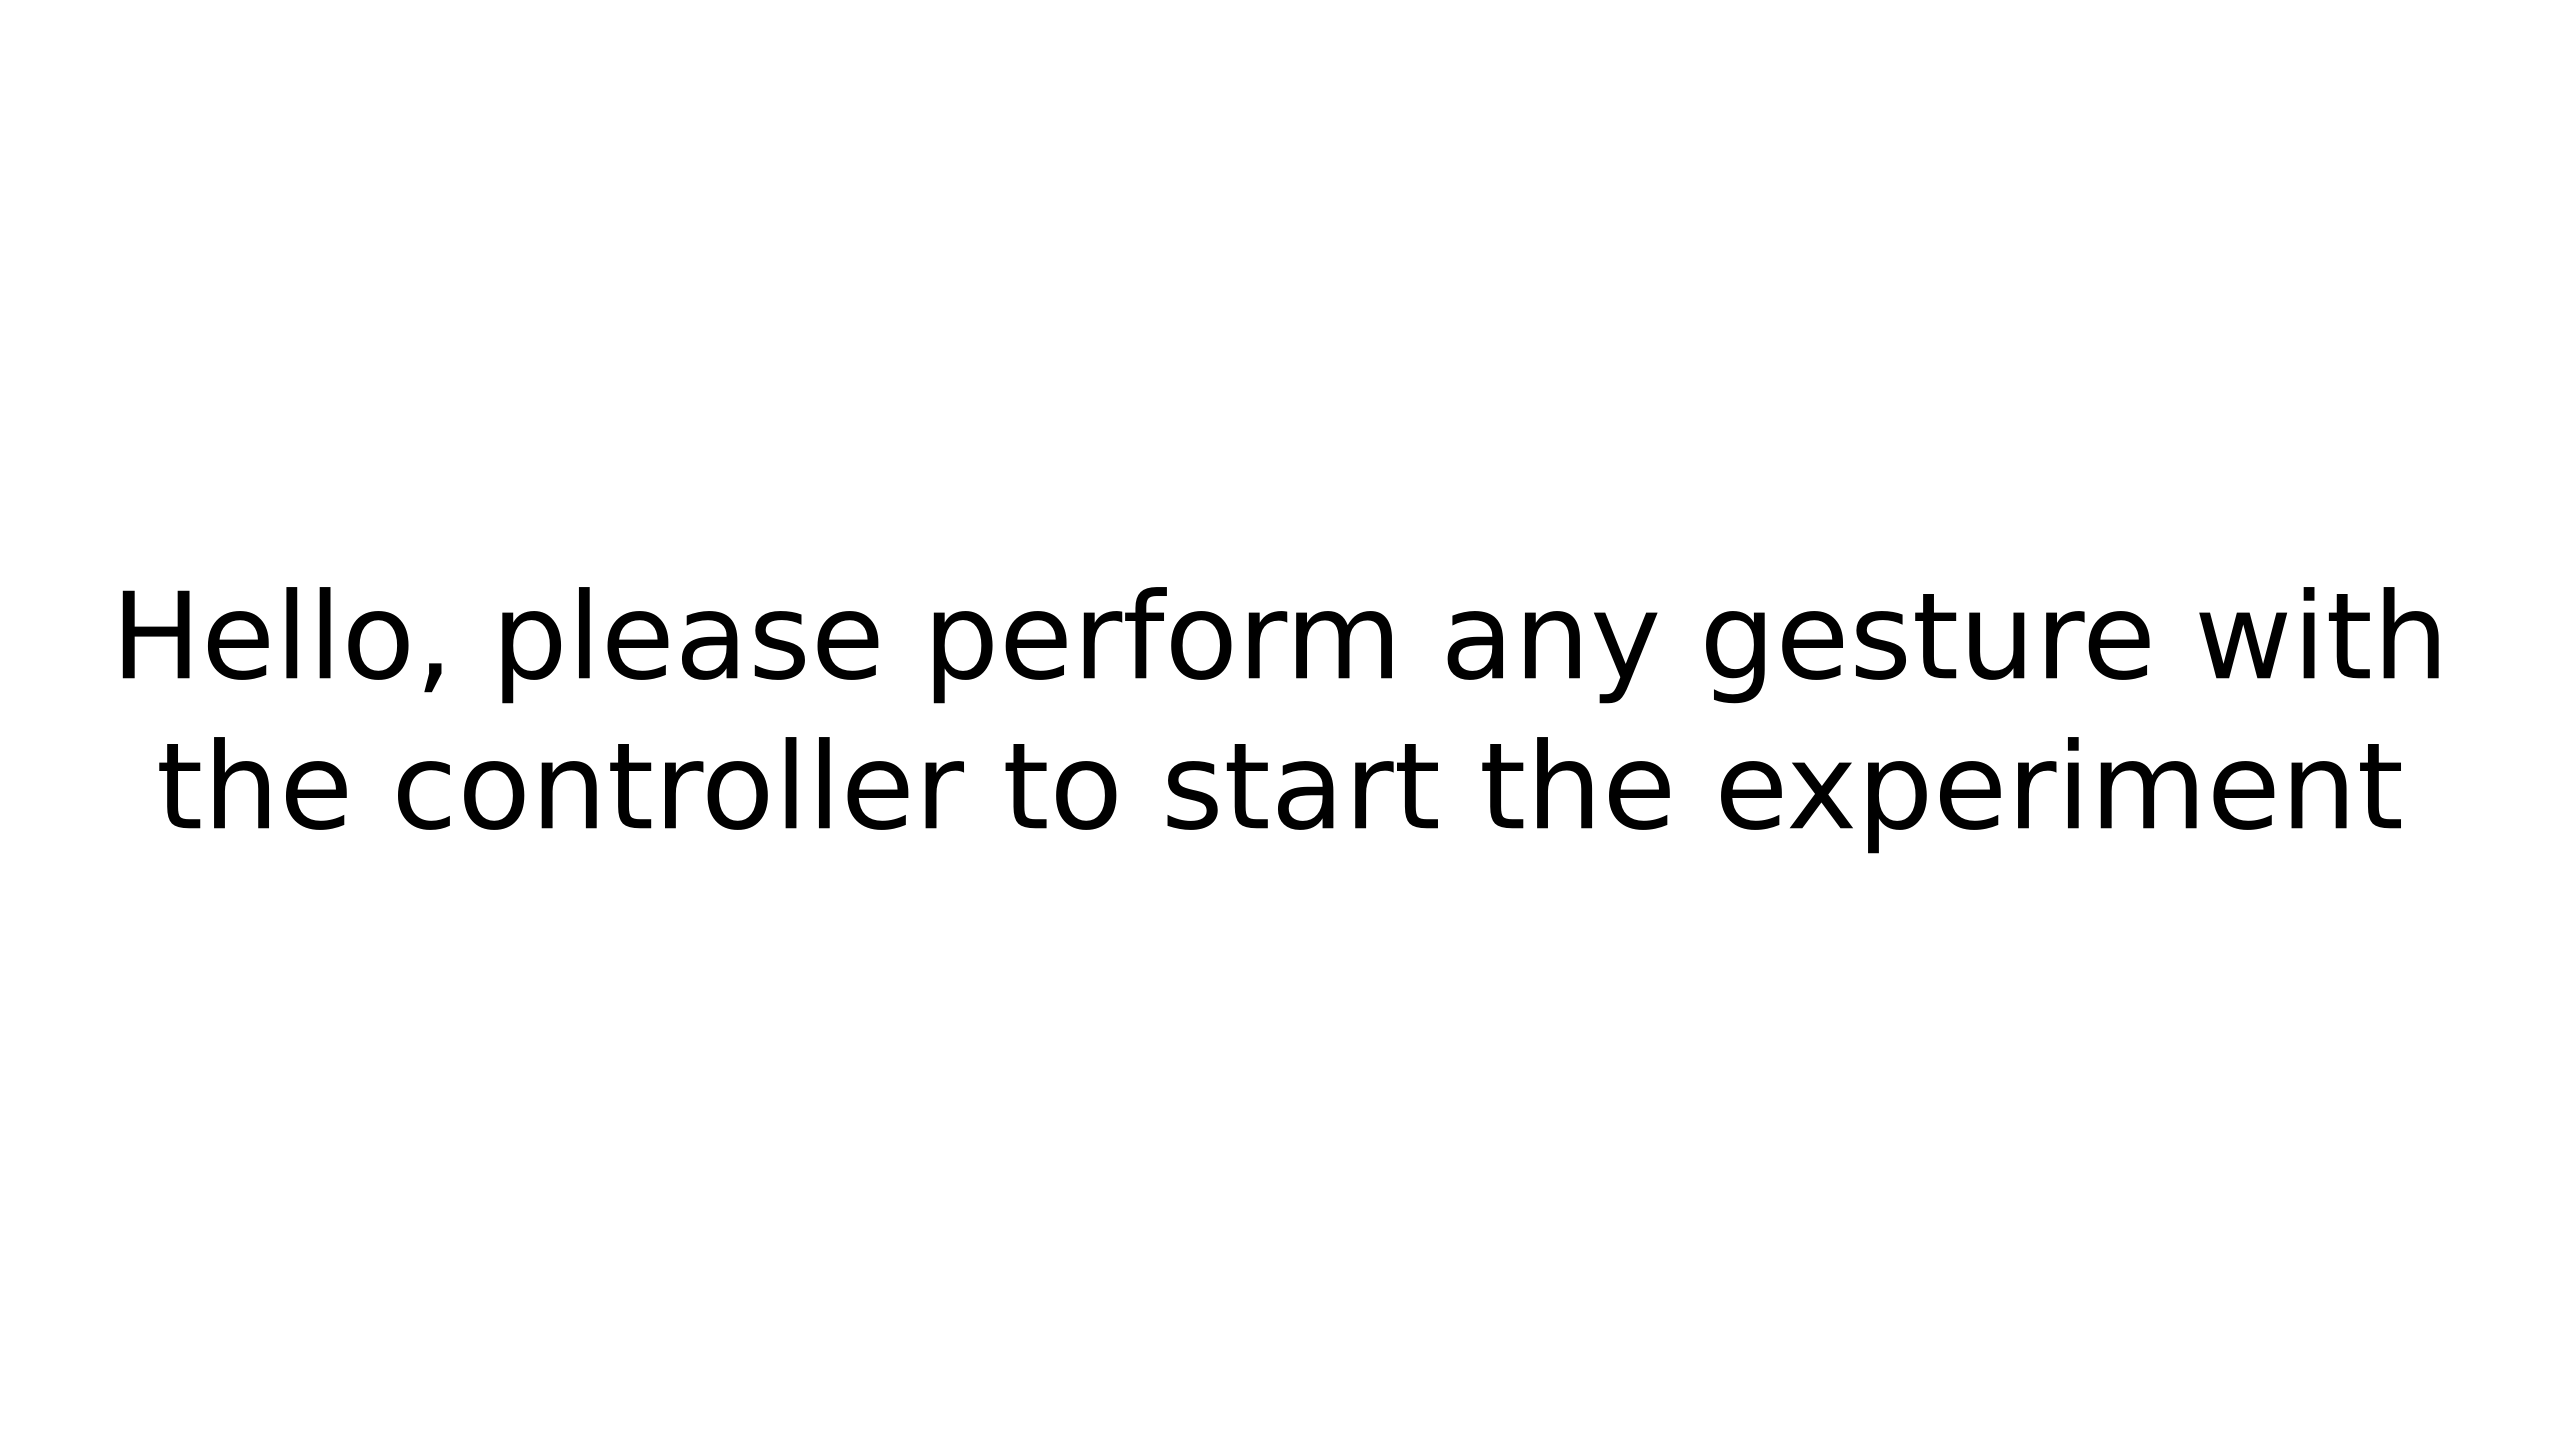
\includegraphics[width=0.3\textwidth]{1.png}} & \frame{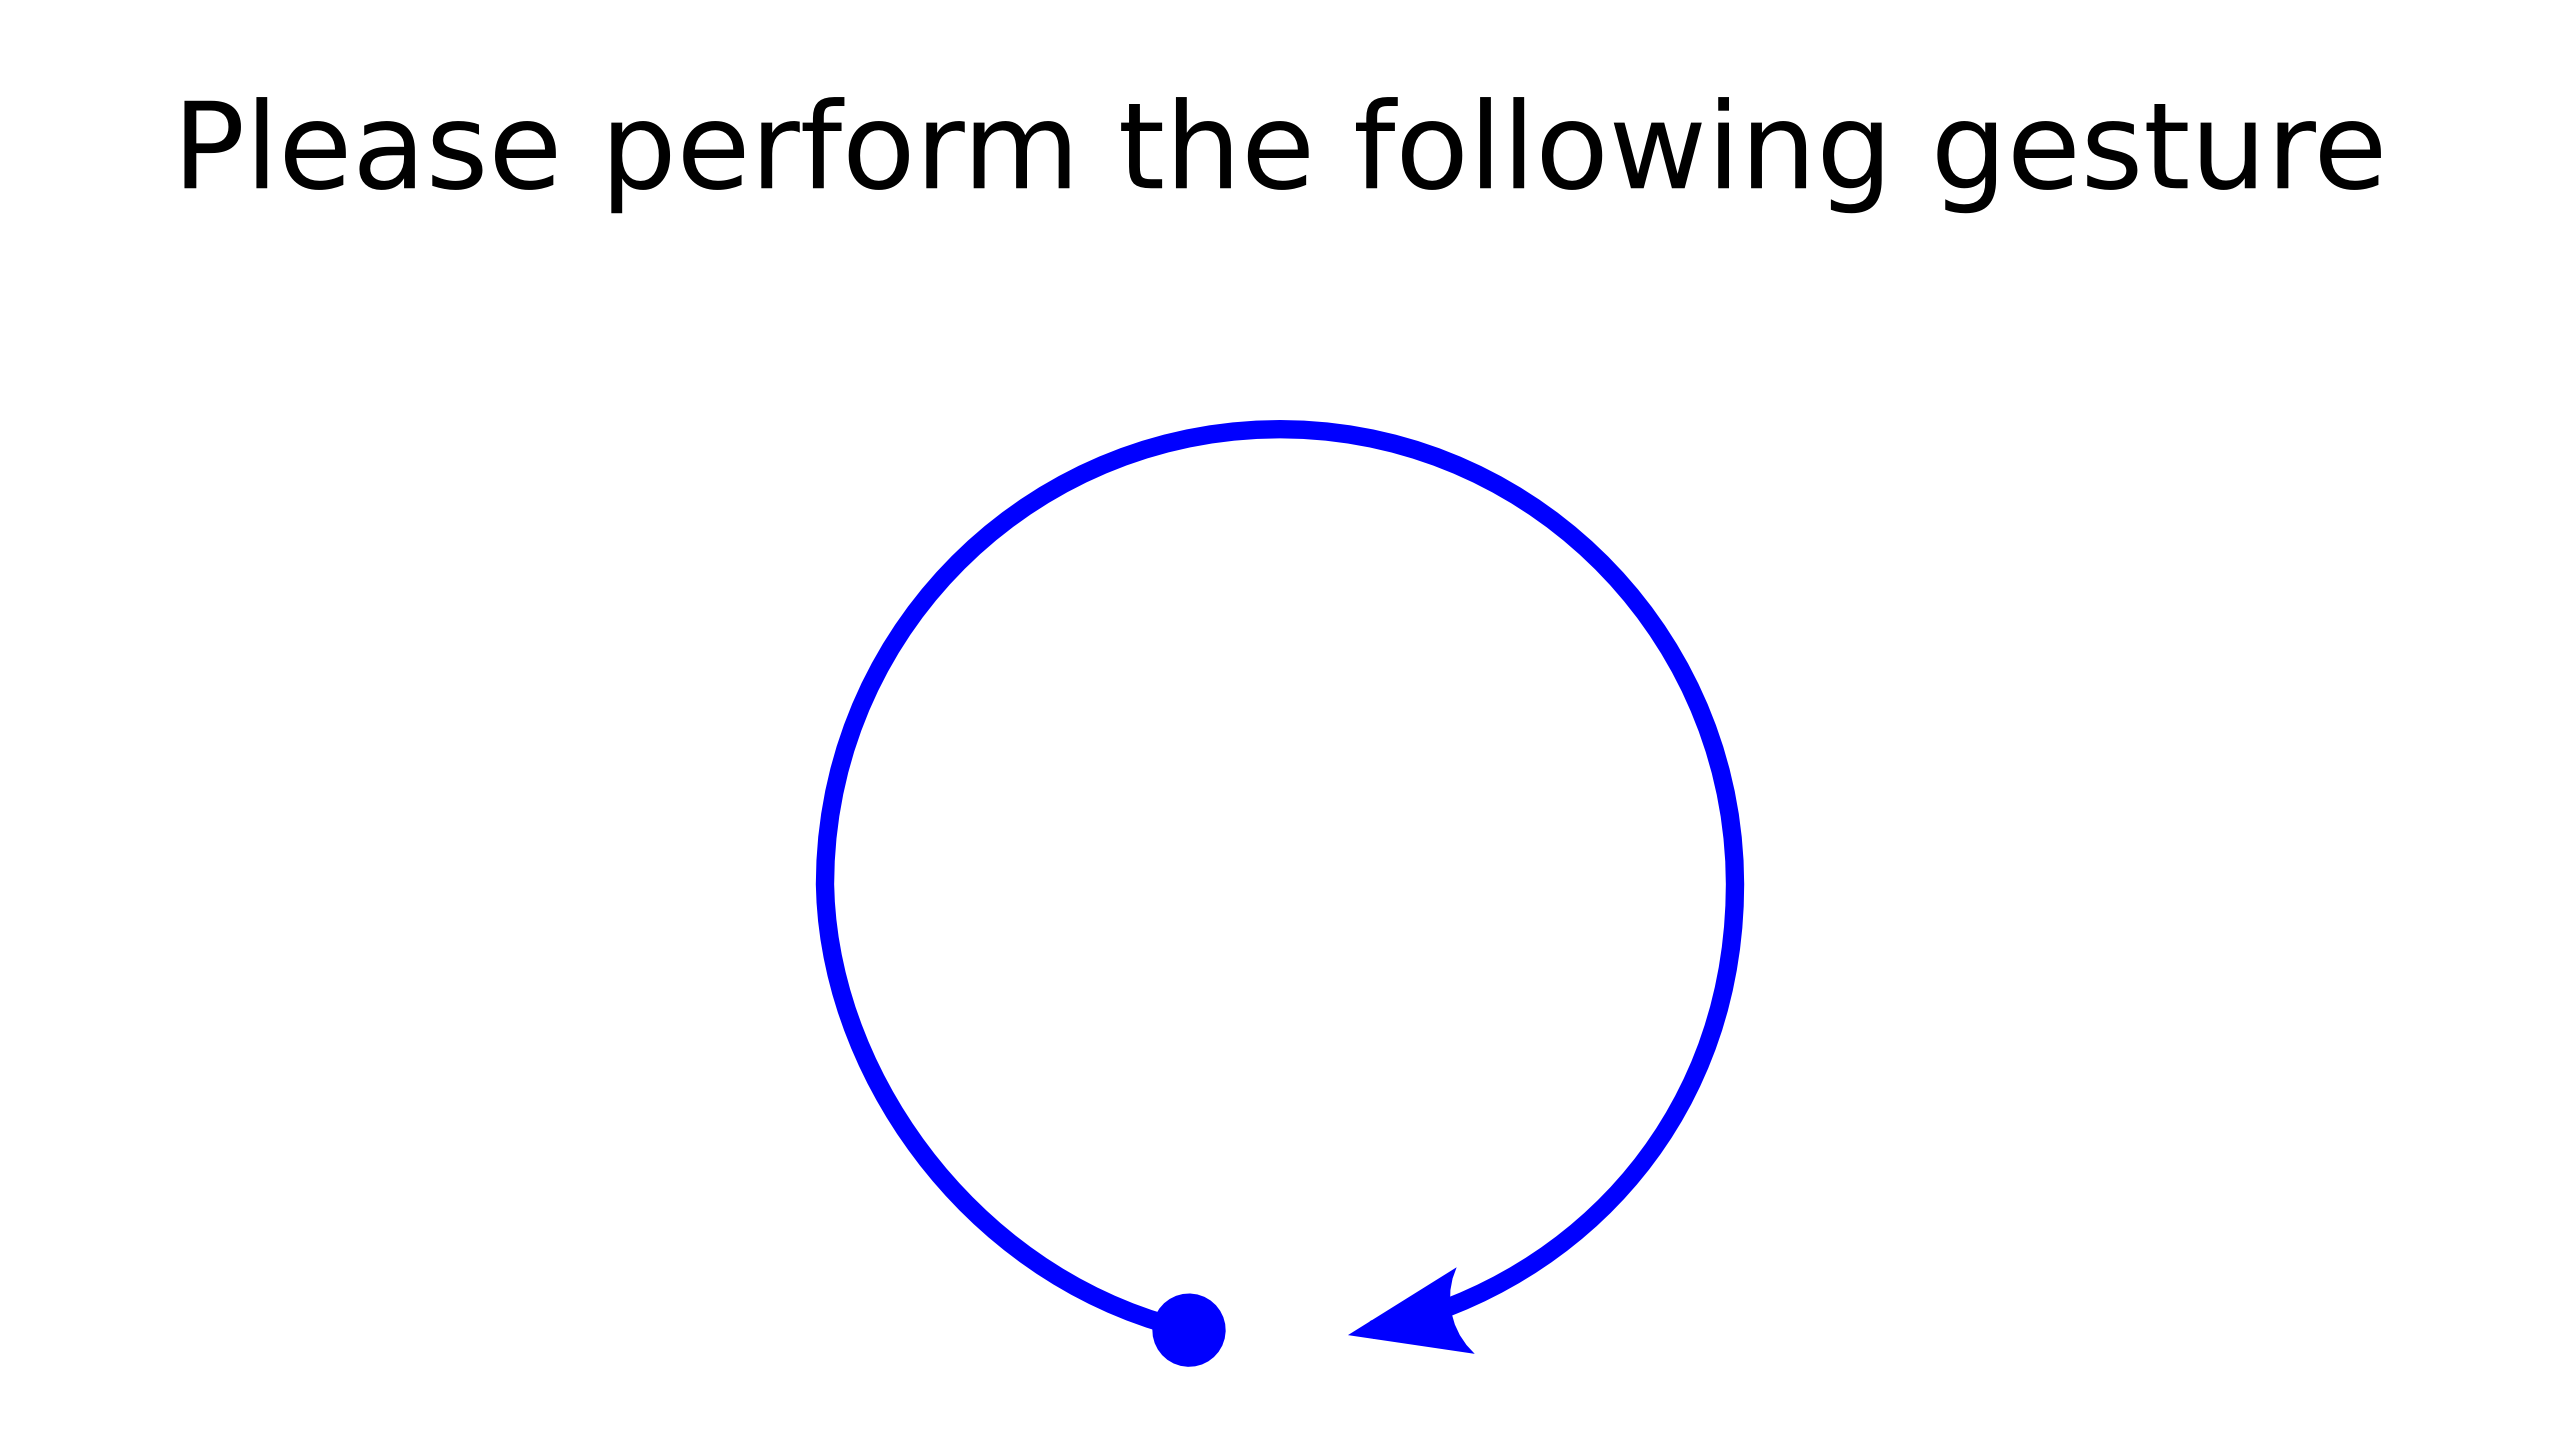
\includegraphics[width=0.3\textwidth]{2.png}} & \frame{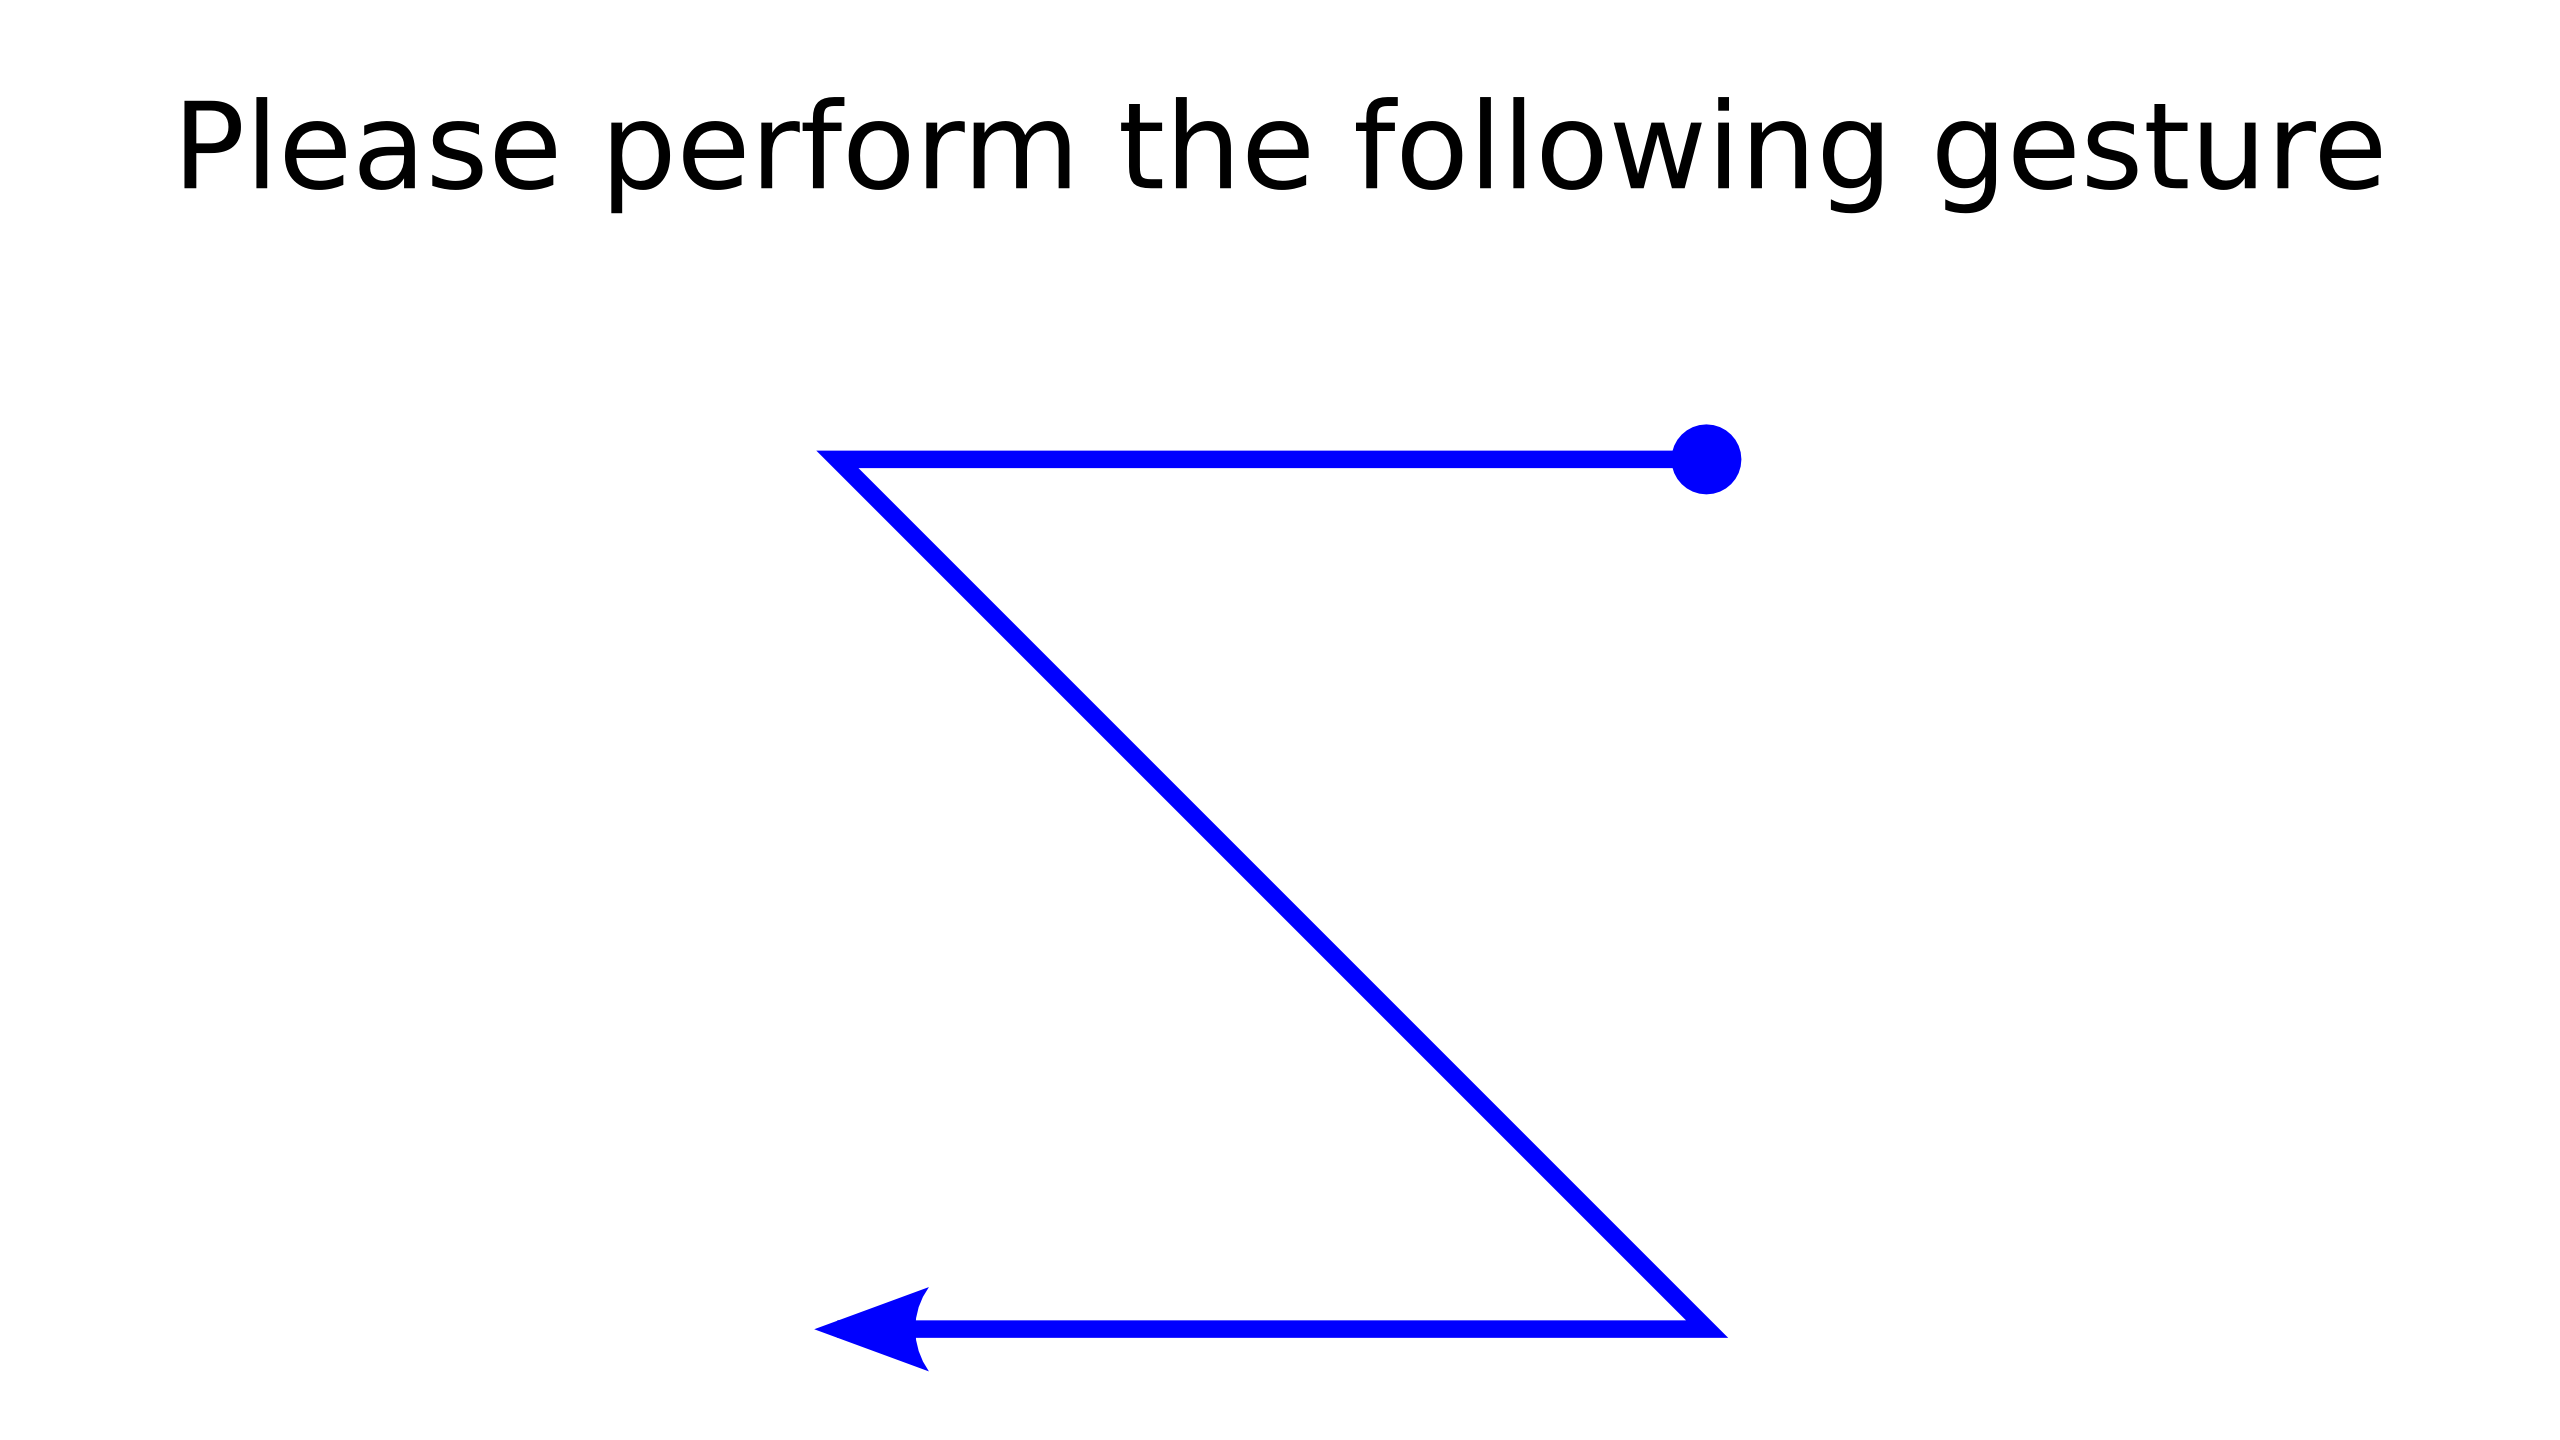
\includegraphics[width=0.3\textwidth]{3.png}} \\
            (a) & (b) & (c) \\
            \frame{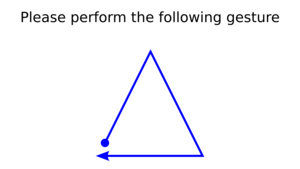
\includegraphics[width=0.3\textwidth]{4.png}} & \frame{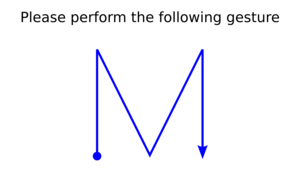
\includegraphics[width=0.3\textwidth]{5.png}} & \frame{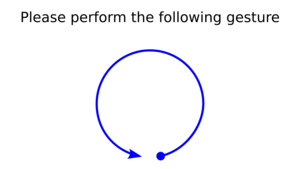
\includegraphics[width=0.3\textwidth]{6.png}} \\
            (d) & (e) & (f) \\
            \frame{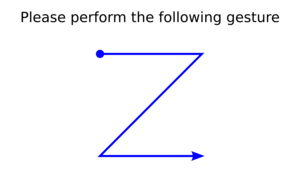
\includegraphics[width=0.3\textwidth]{7.png}} & \frame{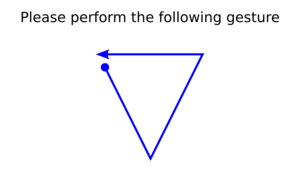
\includegraphics[width=0.3\textwidth]{8.png}} & \frame{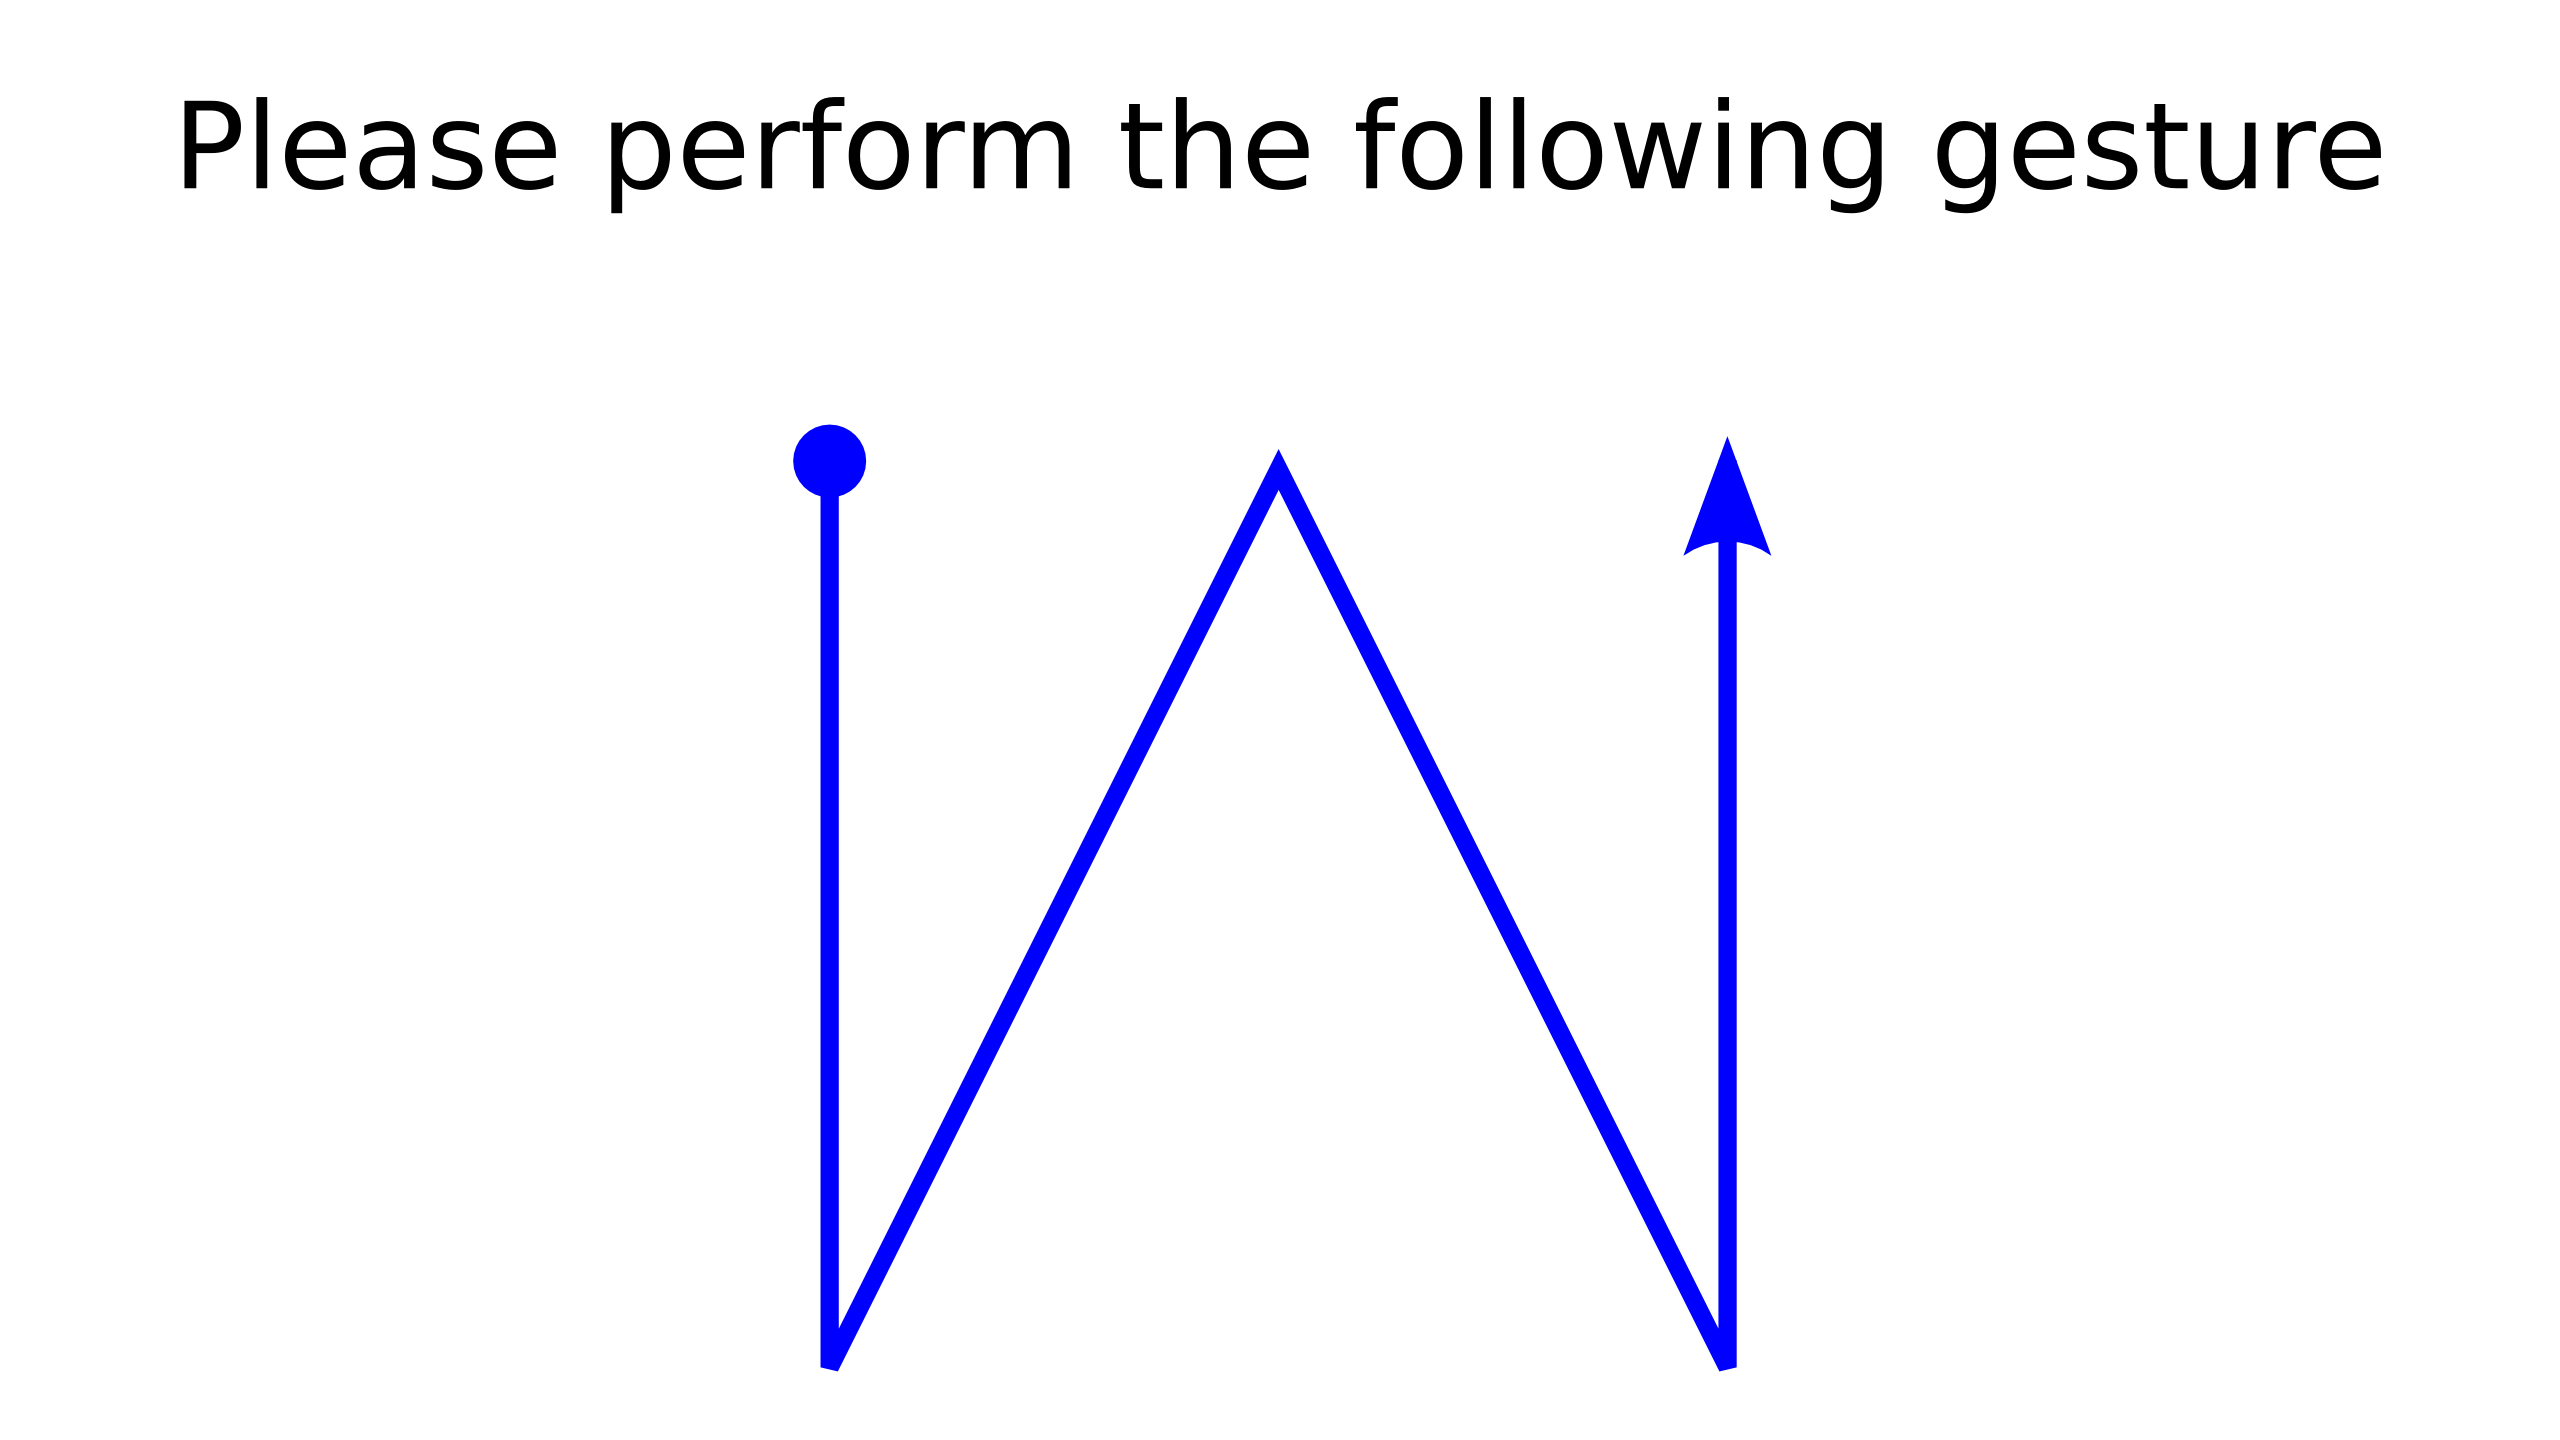
\includegraphics[width=0.3\textwidth]{9.png}} \\
            (g) & (h) & (i) \\
            \frame{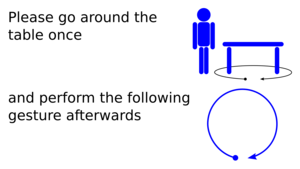
\includegraphics[width=0.3\textwidth]{10.png}} & \frame{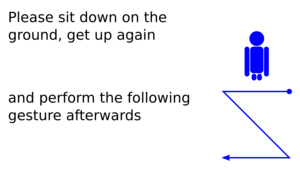
\includegraphics[width=0.3\textwidth]{11.png}} & \frame{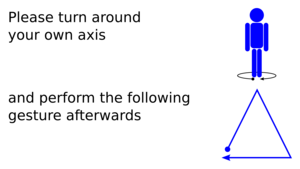
\includegraphics[width=0.3\textwidth]{12.png}} \\
            (j) & (k) & (l) \\
            \frame{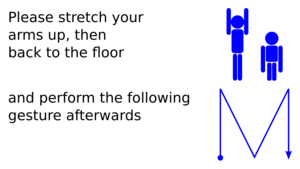
\includegraphics[width=0.3\textwidth]{13.png}} & \frame{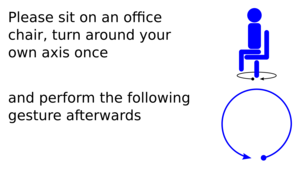
\includegraphics[width=0.3\textwidth]{14.png}} & \frame{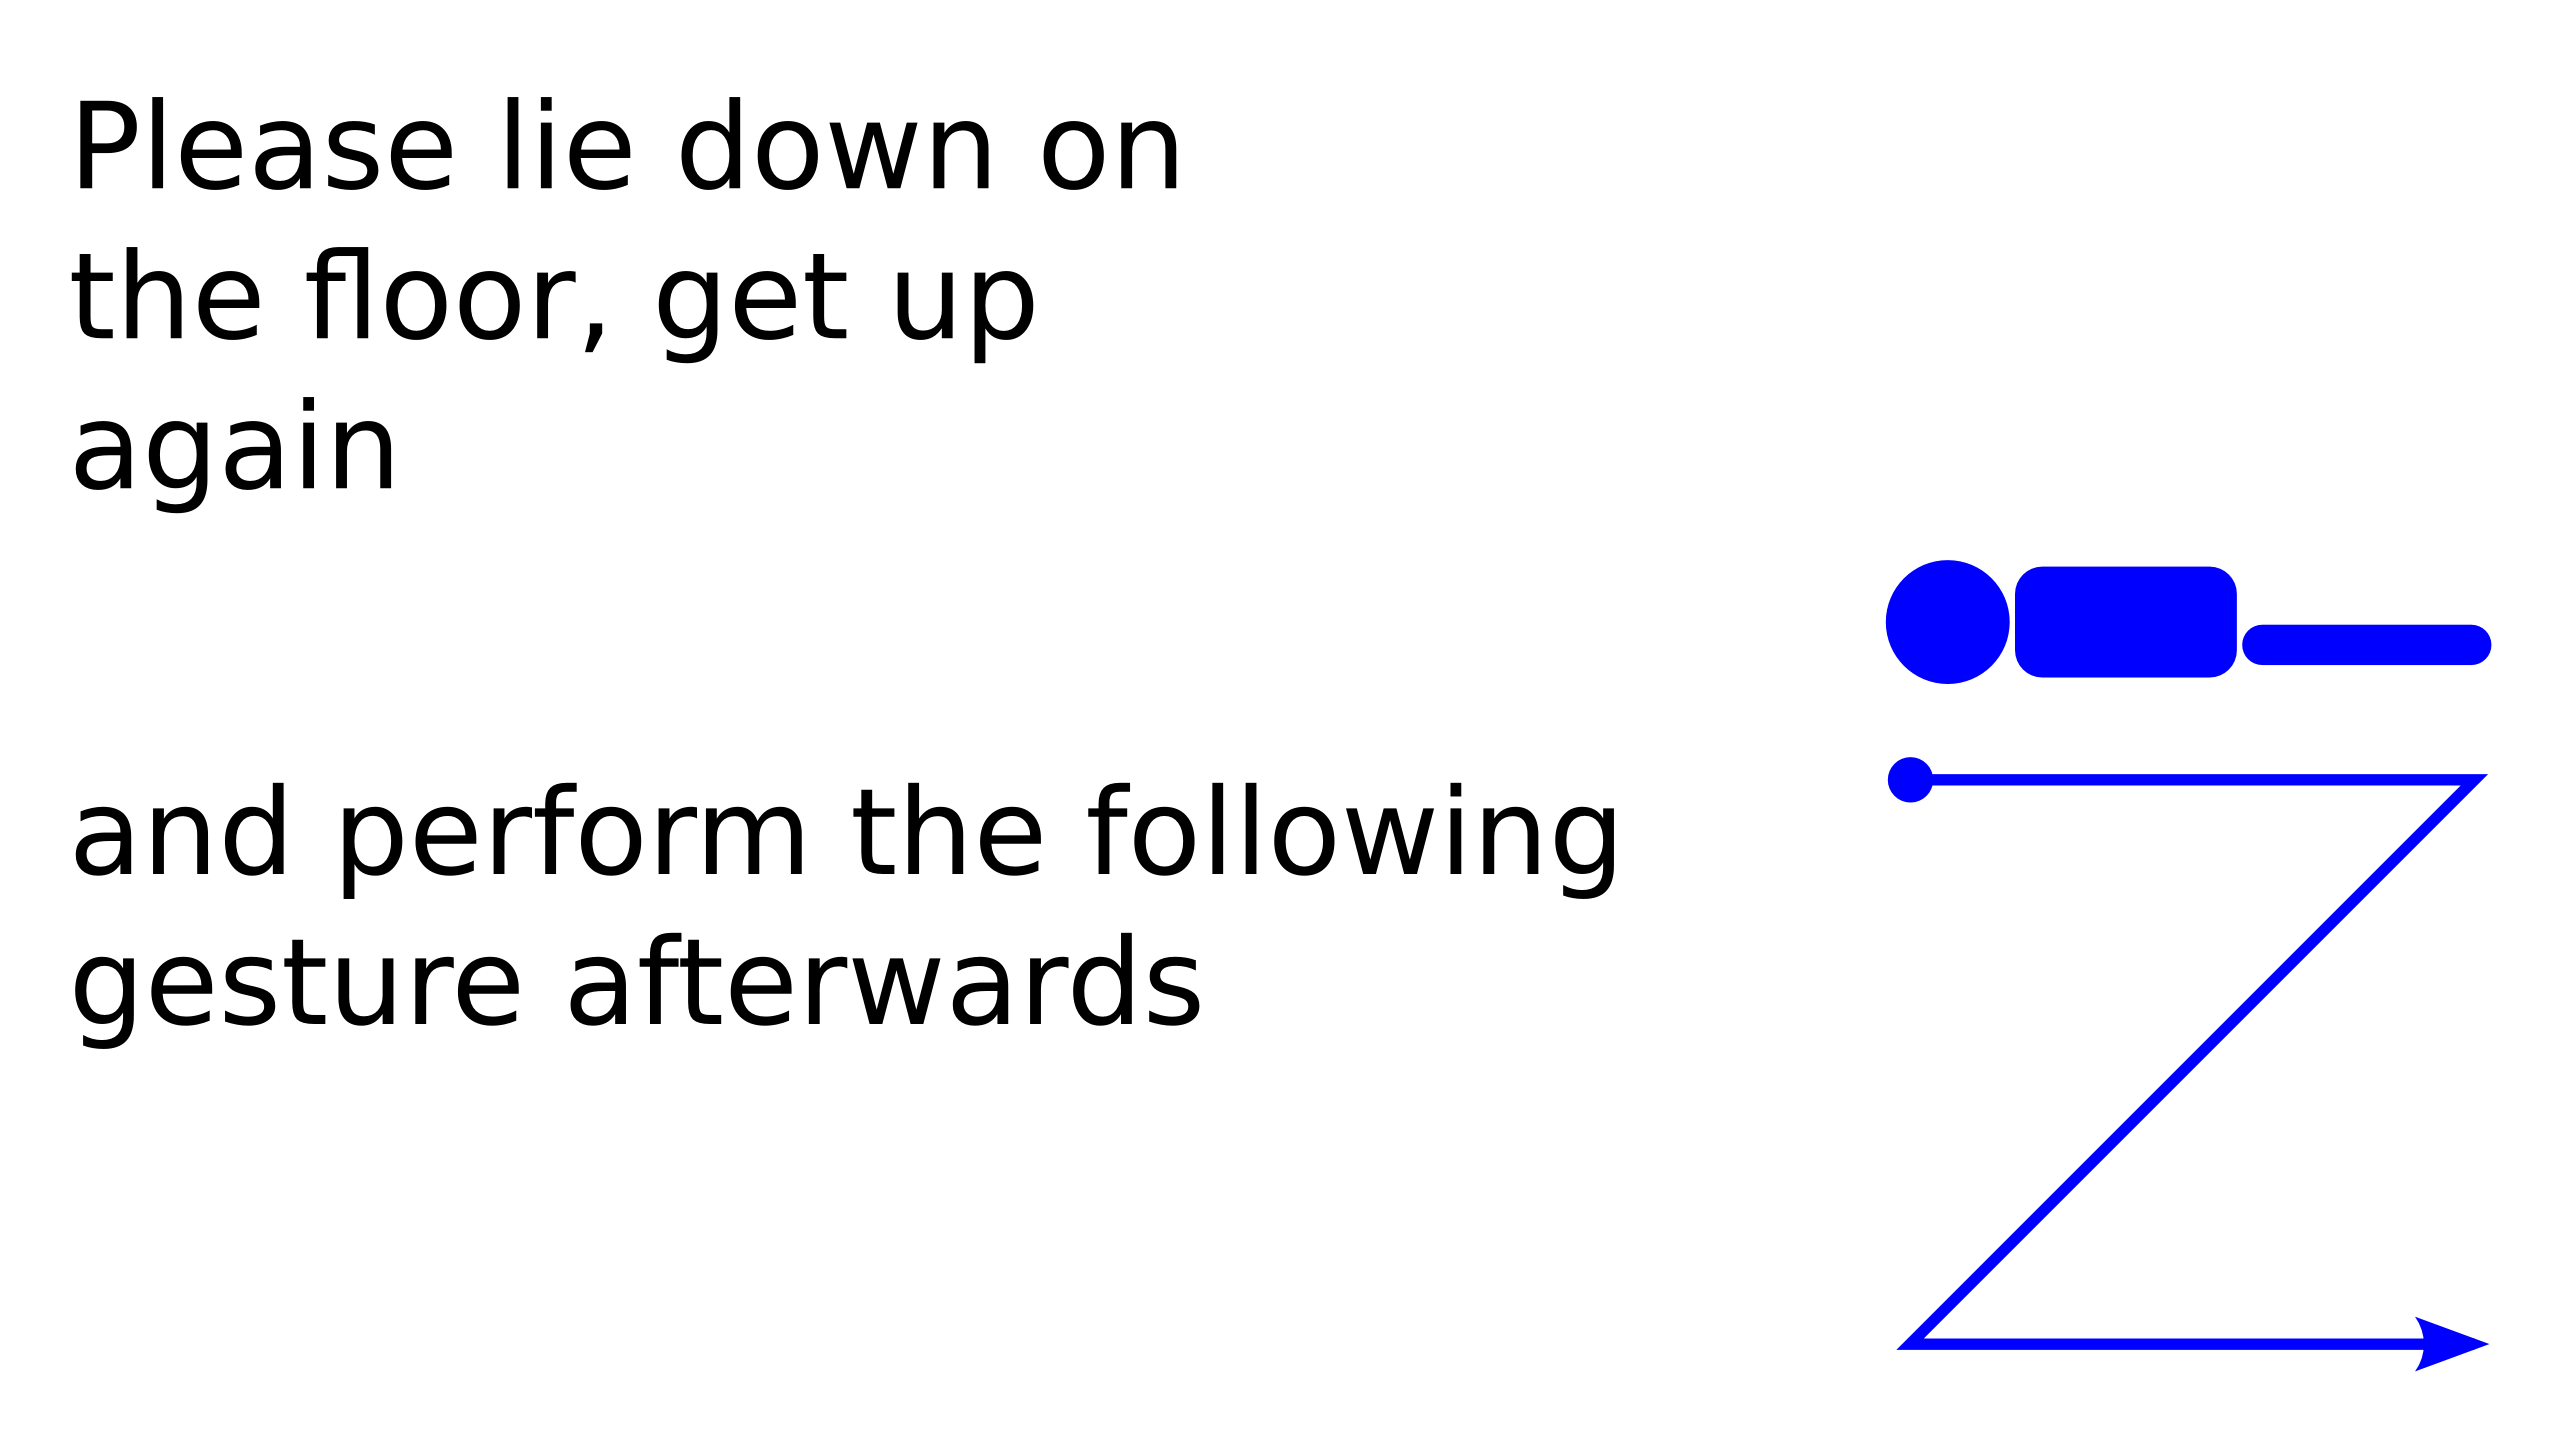
\includegraphics[width=0.3\textwidth]{15.png}} \\
            (m) & (n) & (o) \\
            \frame{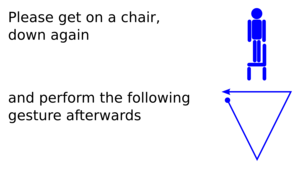
\includegraphics[width=0.3\textwidth]{16.png}} & \frame{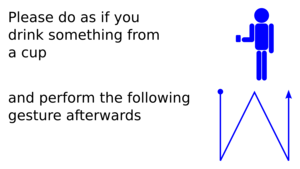
\includegraphics[width=0.3\textwidth]{17.png}} & \frame{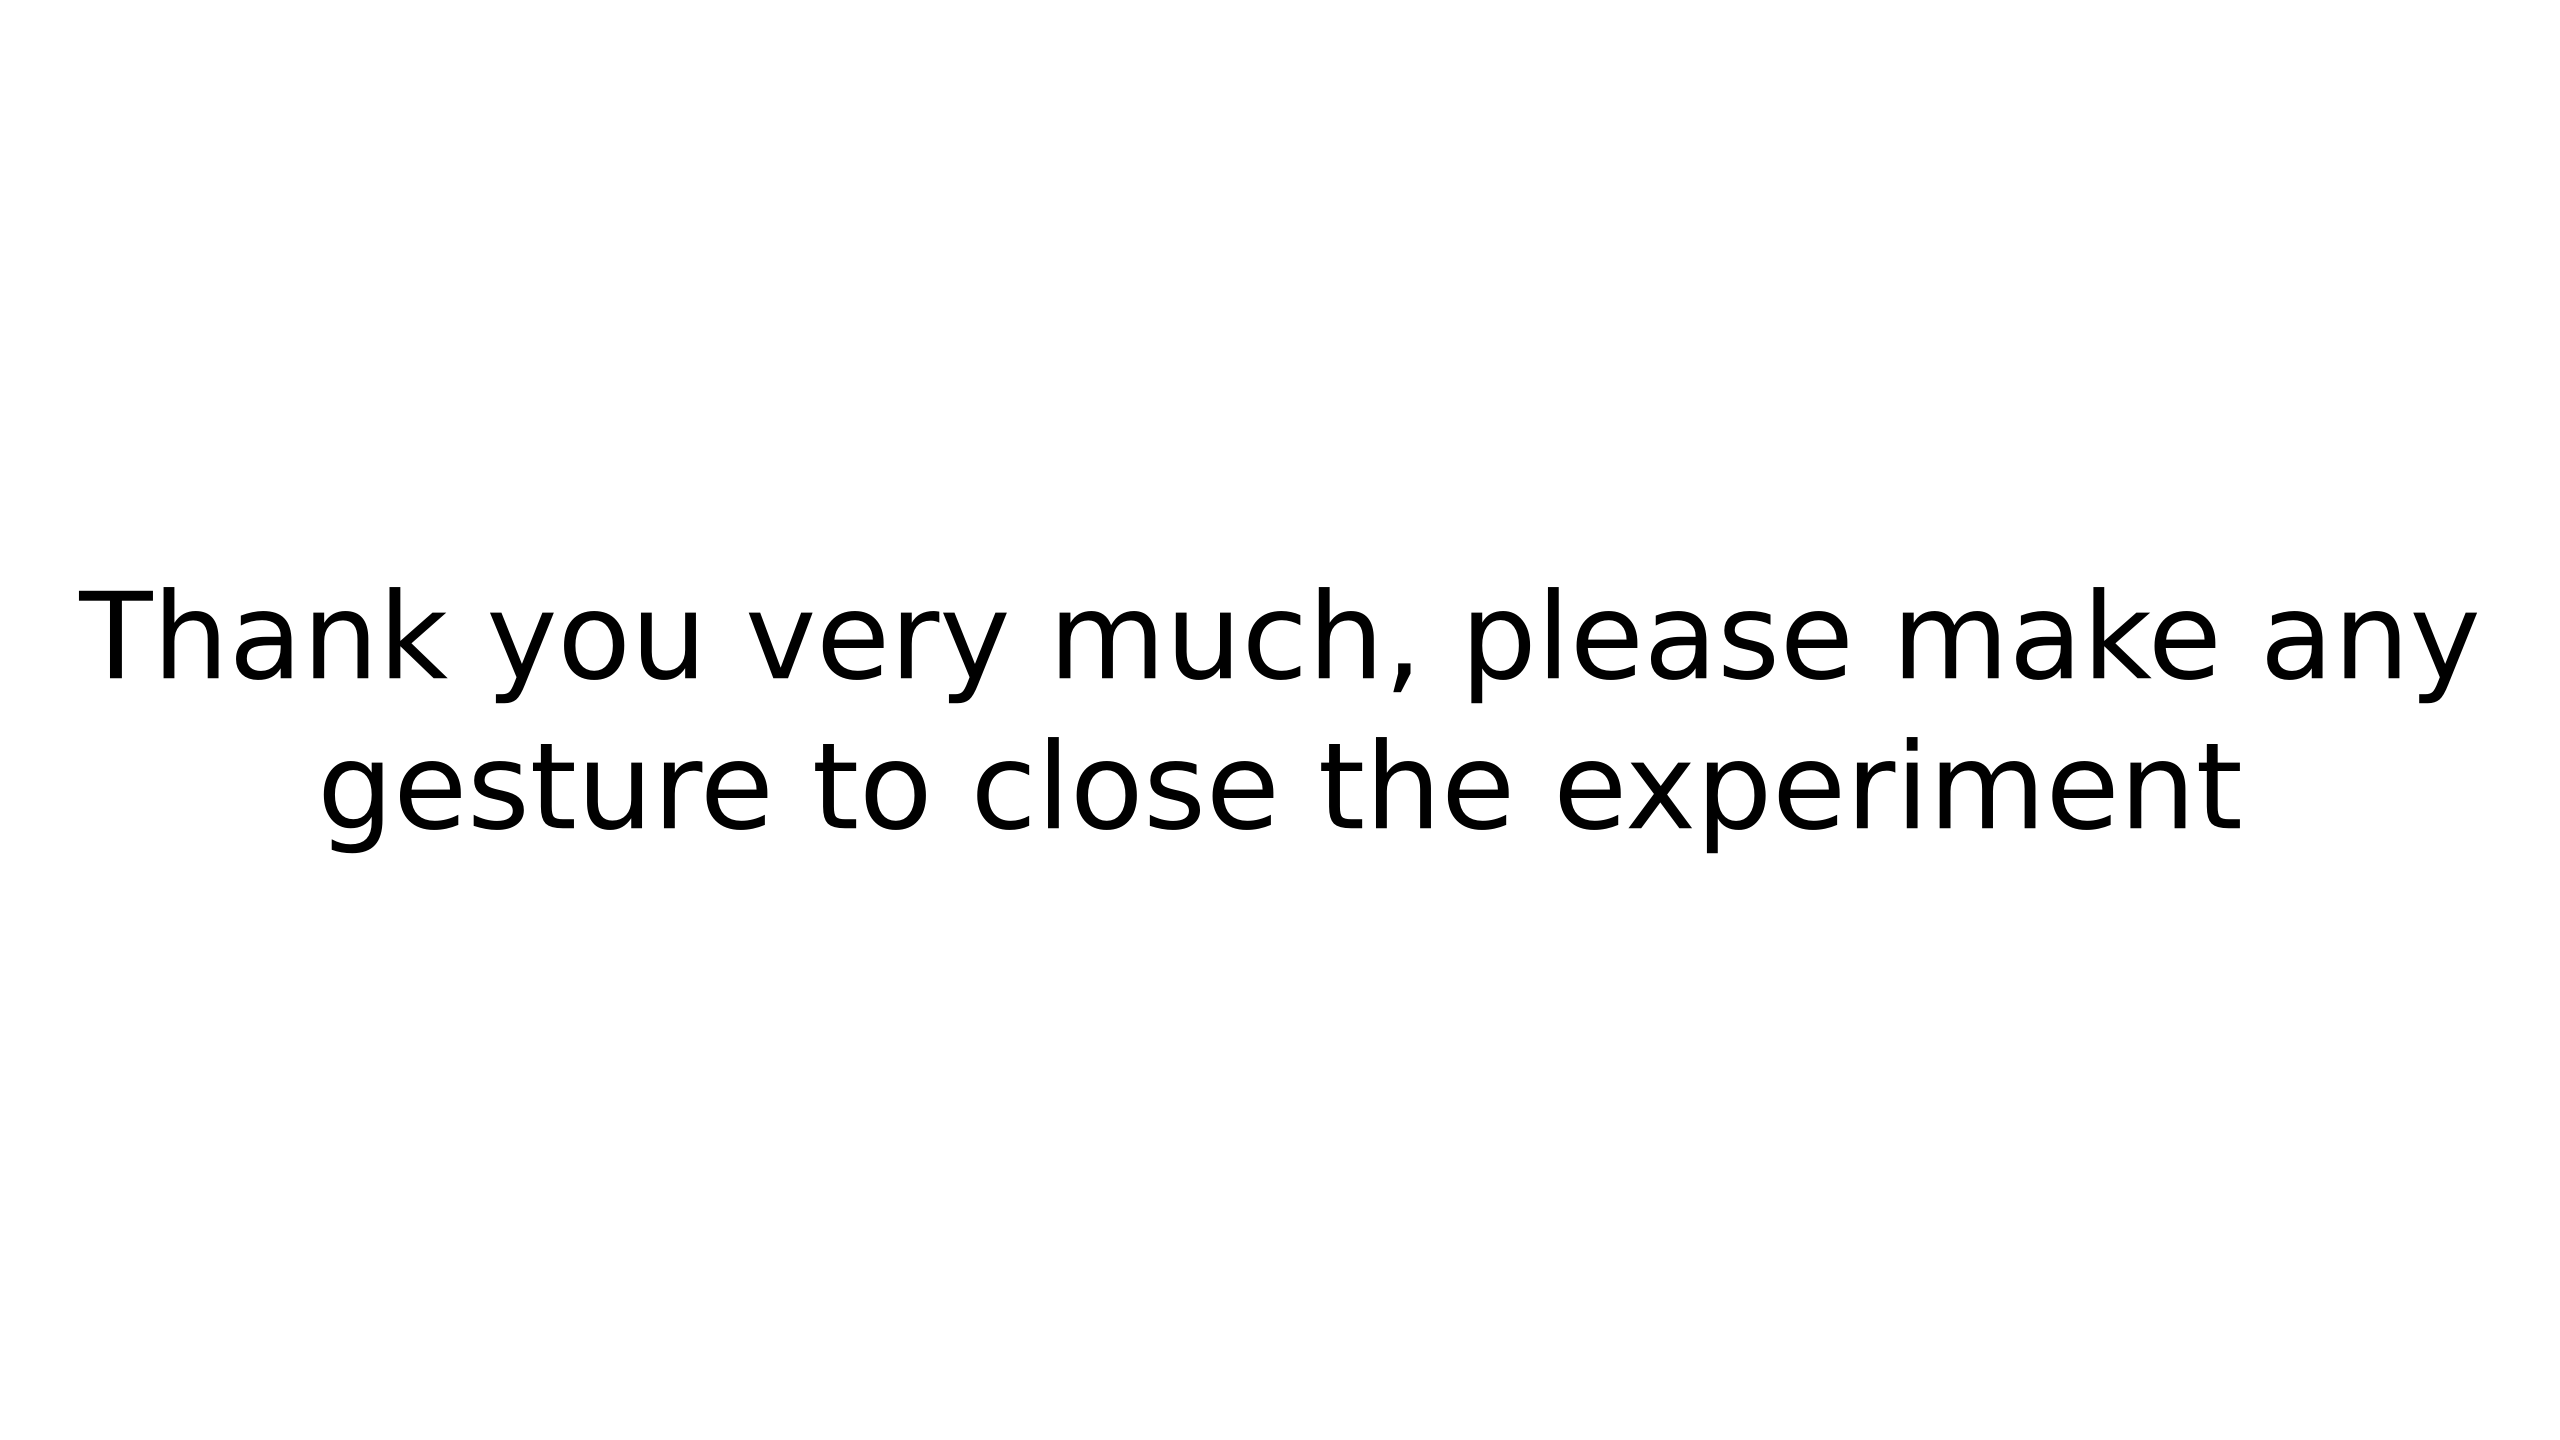
\includegraphics[width=0.3\textwidth]{18.png}} \\
            (p) & (q) & (r) \\
            \multicolumn{3}{c}{\frame{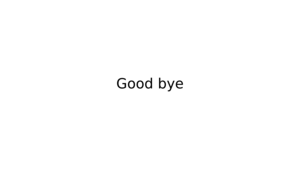
\includegraphics[width=0.3\textwidth]{19.png}}}\\
            \multicolumn{3}{c}{(s)}\\
        \end{tabular}
        \caption{The task screens that will guide the experimentee.}
        \label{fig:screens}
    \end{figure}

    \subsubsection{Data from the experiment}

    The data of an experiment instance is always a file that contains lines of acceleration data and lines of button
    events. Every line will start with the count of milliseconds that have passed since the starting of the experiment.

    \paragraph{Acceleration data} lines contain the count of milliseconds that have passed since the starting of
    the experiment, the \textit{X} value, the \textit{Y} value and the \textit{Z} value of the acceleration data. Here
    an example for a acceleration data line.\\\\
    \verb+33085 -26 -6 89+

    \paragraph{Button down event} lines also contain the count of milliseconds that have passed since the starting
    of the experiment, the keyword \verb+START+ and the index of the gesture in the experiment starting with zero. Here
    an example for a button down event line.\\\\
    \verb+34315 START 4+

    \paragraph{Button up event} lines also contain the count of milliseconds that have passed since the starting
    of the experiment, the keyword \verb+END+ and the index of the gesture in the experiment starting with zero. Here
    an example for a button up event line.\\\\
    \verb+36375 END 4+\\

    The experiment contains nineteen screens and the program is recording from showing the first screen to showing the
    last screen. That means the resulting file will contain eighteen gesture start and end events.

    % Experiementeller Aufbau beschreiben

    %%% SPÄTER
    % Resultate aufzeigen
    % Diskusion mit eigener Interpretation

    % Conclusion
    %% Zukünftiges
    % Future Work
    % References

\end{document}
